\clearpage
\chapter{\textbf{Foundations}}\label{grundlagen}
%\addtocontents{toc}{\vspace{0.8cm}}
\section{Definitions}
\subsection{IoT and IIoT}
The term Internet of Things was first coined by \cite{ashtonThatInternetThings} when explaining the idea of combining RFID with the internet in an executive meeting. He explains that on the "normal" internet, most of the content is created by human beings. In contrast to this in the Internet of Things the data is generated by things and often describes things. But his emphasizes lays more on the description of things. For example to track and count them. The information to do so would come from sensors and RFID, he says.
Of course in these days more of the information on the internet is generated by bots and AI. But other than that the distinction still holds true. 
\\The Internet Society \cite{roseInternetThingsOverview} further explains that in the Internet of Things, machines are communicating with each other and are addressable via an own IP address. This standardizes the way in which devices communicate. They also mention that "Today, the Internet of Things has become a popular term for describing scenarios in which  Internet connectivity and computing capability extend to a variety of objects, devices, sensors, and everyday  items."
\\The Industrial Internet of Things is just the description of a domain where the IoT is used. In this case in manufacturing. \cite{WhatIoTInternet}
\section{State of the Art}\label{unterkapitel}
\subsection{Industrial IoT Architectures and Patterns}
Due to the requirement that the solution be developed utilizing IoT technologies and is set within a production context, a review of Industrial IoT (IIoT) architectures and patterns was conducted. The Industrial Internet Reference Architecture (IIRA) \cite{IIRA} serves as a comprehensive framework, offering valuable insights into various architectural models and design patterns relevant to this domain. This reference architecture describes the following patterns: IoT Component Capability Pattern, Three-Tier Architecture Pattern, Gateway-Mediated Edge Connectivity and Management architecture pattern, Digital Twin Core as a Middleware Architecture Pattern, Layered Databus Architecture Pattern, System-of-Systems Orchestrator Architecture Pattern. Of these patterns only the first two are applicable within the scope of this work. Therefore the other ones will only be described on the surface.
\paragraph{Architecture Patterns}
IoT architecture patterns define the structure and operation of various IoT systems, detailing their implementation and highlighting their unique characteristics.
\subparagraph{IoT Component Capability Model Pattern}
A single component and its associated capabilities are described, with the possibility that a component may comprise multiple sub-components. Consequently, the entire system can also be regarded as a component. The specific meanings of the capabilities are illustrated in the accompanying figure.
\begin{figure}[H]
	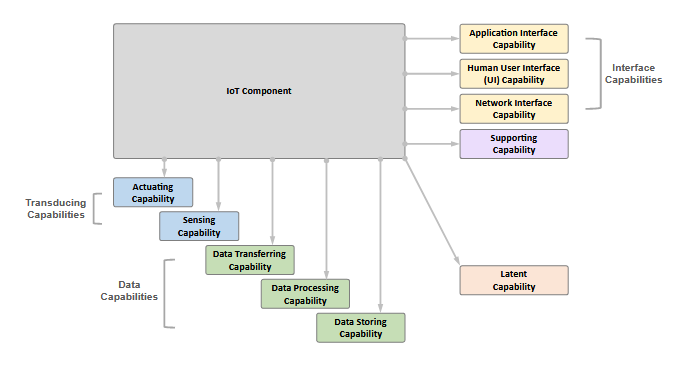
\includegraphics[width=\linewidth]{pic/IIRA-model-component-pattern.png}
	\caption{Component Capability Pattern.}
	\label{fig:Model-Component-Pattern}
\end{figure}
\subparagraph{Three-Tier Architecture Pattern}
The system comprises the Edge, Platform, and Enterprise Tiers, as well as connecting networks. The Edge Tier contains sensors and gateways that collect data. These are connected by the Proximity Network. Data preprocessing may already be happening there.
\\The Platform Tier is responsible for most data processing and storage via databases. It is connected to the Edge Tier via the Access Network.
\\The Enterprise Tier provides domain-specific applications and interfaces for end users. These are built upon the processed data from the platform tier. It also issues controls to lower tiers. This tier is connected to the Access Network via the Service Network.
The three tiers can also be further divided into different domains. That makes sense for bigger systems. But for a symple system as the one described in this work it is not necessary and therefore these domains will be explained here.
\begin{figure}[H]
	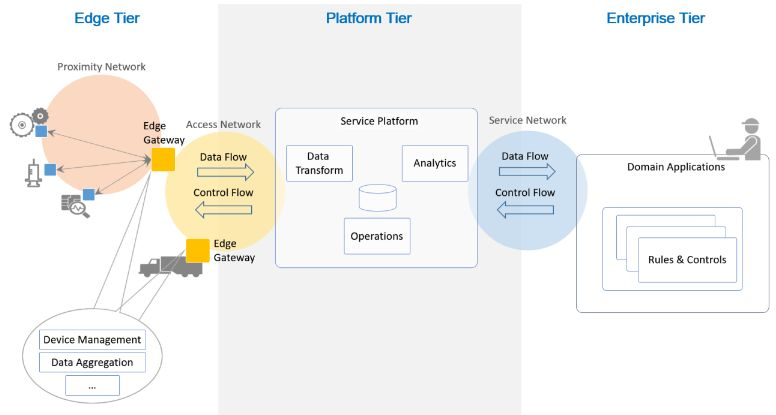
\includegraphics[width=\linewidth]{pic/three-tier-architecture.jpg}
	\caption{Three Tier Architecture}
	\label{fig:Three-Tier-Architecture}
\end{figure}
\subsection{Performance measurement in production environments}
\paragraph{Key Performance Indicators}
The team around \cite{kangHierarchicalStructureKey2016} from the National Institute of Standards and Technologie in the U.S. has worked out the different kinds of KPI's that are being used in operation management and production and how the various metrics and KPI's are related to each other.
\\First there are the supporting elements which in this thesis will be called metrics because they describe the measured data that is needed to calculate the basic KPI's. The supporting elements are devided into the categories time and quantity.
\\Then there are maintenance elements which give insight into upkeep of the machines. Of which the following were able to be calculated with the given metrics.
\\
\subsection{IoT-Plattforms}

\subsection{Databases}
\subsection{Dashboarding}
\addtocontents{toc}{\vspace{0.8cm}}


